%! Author = Ben Gavan
%! Date = 23/02/2021


%%%%%%%%%%%%%% 23/02/2020 %%%%%%%%%%%%%%%%
\subsection*{\textbf{23/02/2020}}
%%%%%%%%%%%%% 9:00 %%%%%%%%%%%%%
\subsubsection*{08:30 - Lead BG}
The ATLAS detector can mistake the production of a $l^+ l^-$ pair from 2 separate decays as pair production from the decay of a single particle, such as a Z boson.
\\
The most probable source of this is from W boson decays:
\begin{align*}
    W^+ \rightarrow l^+ \nu_{l}
    \\
    W^- \rightarrow l^- \Bar{\nu_{l}}
\end{align*}
to be mistaken for $Z \rightarrow ll$.
\\
In the case of $Z \rightarrow ll$, the two leptons would be expected to be produced with the angle between them ($\Delta \phi$) $\approx \pi$ (angle between the azimuthal angle) to conserve momentum.
\\
Counter to this, the  $W^+ \rightarrow l^+ \nu_{l}$ and $W^- \rightarrow l^- \Bar{\nu_{l}}$ can be proceed at any angle, so would expect production to include $\Delta \phi \approx 0$
\\
To investigate this, plot $\Delta \phi$ of ATLAS "2lep" data with the cuts such that - Fig.\ref{fig:2lep_delta-phi_0-7_23-02_09-43}

Fig.\ref{fig:2lep_delta-phi_0-7_23-02_09-43} shows that there is a small peak at lower angles.  This can be produced from. two main processes:
\begin{itemize}
    \item Momentum conservation to compensate for jets
    \item incorrect classification for two W+ and W- decays.
\end{itemize}

Cuts used in Fig.\ref{fig:2lep_delta-phi_0-7_23-02_09-43}:
\begin{lstlisting}
lepCut = "(" + "(lep_charge[0] != lep_charge[1]) && (lep_type[0]==lep_type[1]) && lep_n==2" + ")"
\end{lstlisting}

\begin{figure}[h!]
    \centering
    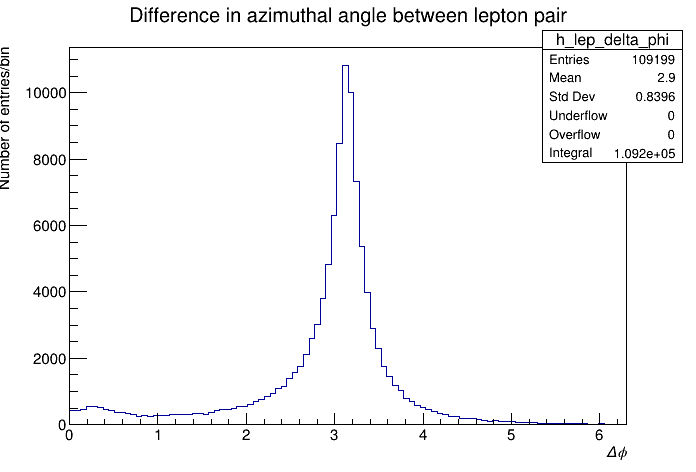
\includegraphics[width=0.85\linewidth]{plots/23-02-2021/2lep_delta-phi_0-7_23-02_09-43.png}
    \caption{The difference of the azimuthal angle of the lepton pair for ATLAS data.  The main peak at approx $\pi$ is as expected.  Cuts: (lep-charge[0] != lep-charge[1]) \&\& (lep-type[0]==lep-type[1]) \&\& lep-n==2}
    \label{fig:2lep_delta-phi_0-7_23-02_09-43}
\end{figure}

Plot the difference between the lepton pair as a stack plot to compare MC and ATLAS data.
\\
Cuts used in Fig.\ref{fig:All-stack-fast_delta-phi_(opp-charge_same-type_n=2)_0-6.3_23-02-21}:
\begin{lstlisting}
lepCut = "(" + "(lep_charge[0] != lep_charge[1]) && (lep_type[0]==lep_type[1]) && lep_n==2" + ")"
\end{lstlisting}

\begin{figure}[h!]
    \centering
    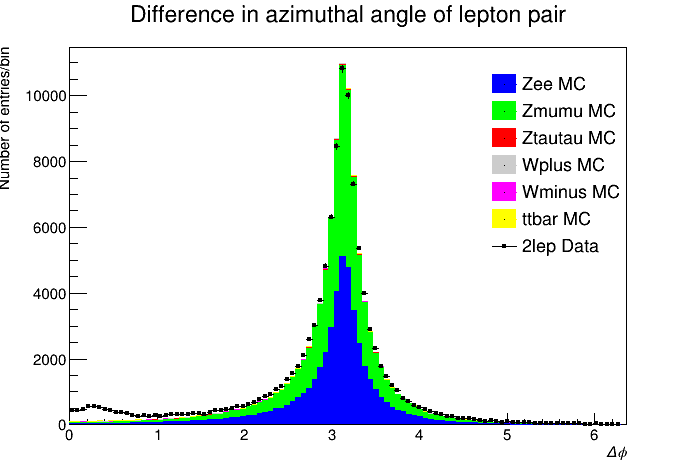
\includegraphics[width=0.85\linewidth]{plots/23-02-2021/All-stack-fast_delta-phi_(opp-charge_same-type_n=2)_0-6.3_23-02-21.png}
    \caption{The difference of the azimuthal angle of the lepton pair for ATLAS data with MC data stacked (included main MC simulated background and source).  The main peak at approx $\pi$ is as expected.  Cuts: (lep-charge[0] != lep-charge[1]) \&\& (lep-type[0]==lep-type[1]) \&\& lep-n==2}
    \label{fig:All-stack-fast_delta-phi_(opp-charge_same-type_n=2)_0-6.3_23-02-21}
\end{figure}


%%%%%%%%%% Plot focussing on electron pair

\begin{figure}[h!]
    \centering
    \begin{minipage}{0.5\textwidth}
        \centering
        \includegraphics[width=\linewidth]{plots/}
        (A)
    \end{minipage}\hfill
    \begin{minipage}{0.5\textwidth}
        \centering
        \includegraphics[width=\linewidth]{plots/}
        (B)
    \end{minipage}
    \caption{(A) (B)}
    \label{fig:}
\end{figure}


%%%%%%%%%% Plot focussing on muon pair


%%%%%%%%%% Add invar mass cuts (electron and muon pair side my side - and then both)

Plotting the same data with the same cuts as for Fig.\ref{fig:2lep_delta-phi_0-7_23-02_09-43} in the form of a stack plot to show expected contributions from signal and background sourced using MC data.

\subsubsection*{09:48 - Lead DG}
Apply ptcone20 cut on invariant mass plots.
\\
Since there is no distinction between events in the range 0-1 GeV, cut events above 1 GeV.
\\
Since variables/quantities are correlated (can be effected by the same physical process), plot the etcone20 stack plot.   See Fig.\ref{}


\subsubsection*{12:21}
Plot



\subsection*{14:07 - Lead BG}
Plot pT log to test for potential cuts.

Test other kinematic variables to look for potential cuts

Upper bound cut of 320GeV for total lepton pair pT.  See Fig.{}

\subsection*{15:24 - Lead DG}
Plot eta in search of potential cuts.
\\
Decide on upper cut of $\eta- 2.5$ using Fig.\ref{}


\subsection*{15:31}
Plot the stack plot of delta phi in search of possible cuts.
\\
First apply only minimal cuts (no lower from invariant mass and upper ):
\begin{lstlisting}
    ...
\end{lstlisting}
\begin{figure}[h!]
    \centering
    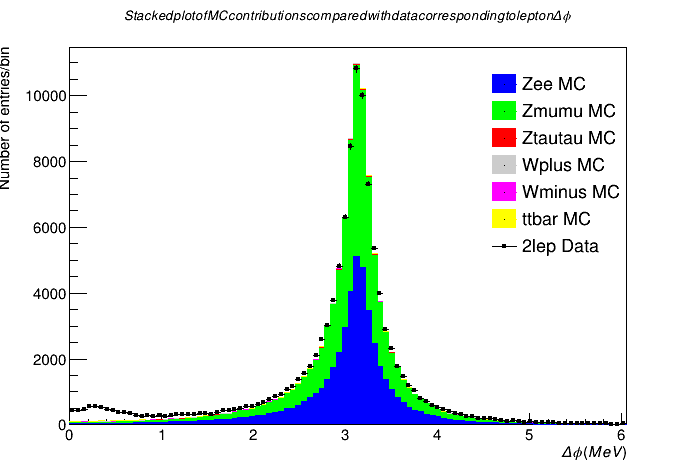
\includegraphics[width=0.85\linewidth]{plots/23-02-2021/All-stack-fast_delta-phi_minimal-cuts_0-6_23-02-21_15-30.png}
    \caption{Stack plot of delta phi with only minimal cuts to select for events with 2 leptons of same type with opposite charge.  There is an inconsitancy between MC and ATLAS data}\label{fig:All-stack-fast_delta-phi_minimal-cuts_0-6_23-02-21_15-30}
\end{figure}
From Fig.\ref{fig:All-stack-fast_delta-phi_minimal-cuts_0-6_23-02-21_15-30}:
- Inconstancy between MC and ATLAS data around 0-1 rad.

Now add upper from total transverse momentum and lower from invariant mass.
\begin{figure}[h!]
    \centering
    \includegraphics[width=0.85\linewidth]{plots/}
    \caption{Stack plot of delta phi with only minimal cuts to select for events with 2 leptons of same type with opposite charge.  There is an inconsitancy between MC and ATLAS data}\label{fig:All-stack-fast_delta-phi_minimal-cuts_0-6_23-02-21_15-30}
\end{figure}
From Fig.\ref{}:
-> Good MC fit to ATLAS data - no more "bump" between 0-1 rad

Question: Is it better to make cuts based on individual particles or total/mean.


\subsection*{15:54 - Lead BG}
Start to calculate the cross section of $pp \rightarrow Z \rightarrow ee$ with the new cuts (lower and upper bounds on variables).
\\
Cuts being used:
\begin{lstlisting}
lepCut ="(" + "(lep_charge[0] != lep_charge[1]) && (lep_type[0]==lep_type[1]) && lep_n==2 && (inv_mass_Zll > 60e3) && (lep_pt[0]+lep_pt[1]) < 320e3 " + ")"
\end{lstlisting}

